\chapter{Initial Baseline Results}
\label{ch:results}

Numbers are means over samples (PSNR in dB / SSIM); the number of samples is given in each table. The Gaussian and
grid methods always use identical measurements and data terms. Initial runs (October 2026) used three samples; the
final runs (November 2026) used five samples for 2D scattering and added the experiments marked as final.

\section{Representation check}
Fitting Gaussians directly to the ground truth (no physics) confirms that the representation can express the
fields: 48.2\,dB / 0.998 on the 2D cells with about 680 Gaussians, and 65.2\,dB / 0.999 on the synthetic 3D volumes
with 5500 Gaussians.

\section{2D inverse scattering on InverseBench cells}
\label{sec:ghost}
Table~\ref{tab:s2d} lists the reconstructions from measurements only. Without regularisation, Gaussians are 6--7\,dB
below the pixel grid with 360 or 180 receivers and 2.7\,dB below with 60. Increasing the Gaussian budget did
\emph{not} help: with aggressive densification (about 2000 Gaussians) PSNR fell to 22.9 / 22.6 / 19.6\,dB. The
reconstructions show why (Figure~\ref{fig:ghost}): a faint copy of the cell appears outside the object. These
``ghosts'' sit where the back-projected residual is large but the measurements carry almost no information, so the
data term cannot remove them (Chapter~\ref{ch:formulation}). Adding the sparsity term removes the ghosts. With
$\lambda=0.3$ Gaussians improve at every receiver count, and at 60 receivers they exceed the unregularised pixel
grid in SSIM (0.924 vs.\ 0.886 over five samples; 0.940 vs.\ 0.878 over the first three) while staying 1--1.5\,dB lower
in PSNR. Larger weights ($\lambda=1,3$) shrink the cells and lower both metrics; $\lambda=0.1$ gives slightly higher
PSNR than 0.3 at 360 and 180 receivers.

The final runs add a \emph{fair} baseline: the pixel grid with the same sparsity term. It reaches 27.7\,dB / 0.933 at
60 receivers and exceeds the Gaussians in both metrics at every receiver count. The SSIM advantage at 60 receivers
therefore comes from the sparsity prior, not from the Gaussian representation itself. Sparsity is, however,
\emph{necessary} for Gaussians (it prevents ghosts) while it costs the grid PSNR at high receiver counts
(36.1 $\to$ 33.2\,dB at 360).

\begin{table}[h]
  \centering
  \caption{2D inverse scattering, InverseBench cells (PSNR dB / SSIM).}
  \label{tab:s2d}
  \resizebox{\linewidth}{!}{%
  \begin{tabular}{llccc}
    \toprule
    & Method & 360 receivers & 180 receivers & 60 receivers \\
    \midrule
    \multirow{6}{*}{\shortstack[l]{Initial\\(3 samples)}}
    & Gaussians & 30.7 / 0.959 & 30.4 / 0.957 & 26.5 / 0.814 \\
    & Gaussians, $\sim$2000 (aggressive densification) & 22.9 / -- & 22.6 / -- & 19.6 / -- \\
    & Gaussians + sparsity, $\lambda=0.3$ & 31.4 / 0.983 & 31.0 / 0.982 & 28.2 / 0.940 \\
    & Gaussians + sparsity, $\lambda=1$ & 27.6 / 0.958 & 27.6 / 0.958 & 25.2 / 0.908 \\
    & Gaussians + sparsity, $\lambda=3$ & 21.6 / 0.875 & 21.6 / 0.876 & 20.5 / 0.826 \\
    & Pixel grid & 36.7 / 0.985 & 35.3 / 0.976 & 29.2 / 0.878 \\
    \midrule
    \multirow{4}{*}{\shortstack[l]{Final\\(5 samples)}}
    & Gaussians + sparsity, $\lambda=0.1$ & 31.8 / 0.982 & 31.5 / 0.980 & 27.4 / 0.909 \\
    & Gaussians + sparsity, $\lambda=0.3$ & 30.8 / 0.980 & 30.6 / 0.979 & 27.1 / 0.924 \\
    & Pixel grid & \textbf{36.1} / 0.984 & \textbf{34.7} / 0.974 & \textbf{28.6} / 0.886 \\
    & Pixel grid + sparsity, $\lambda=0.3$ & 33.2 / \textbf{0.985} & 32.5 / \textbf{0.983} & 27.7 / \textbf{0.933} \\
    \bottomrule
  \end{tabular}}
\end{table}

\begin{figure}[h]
  \centering
  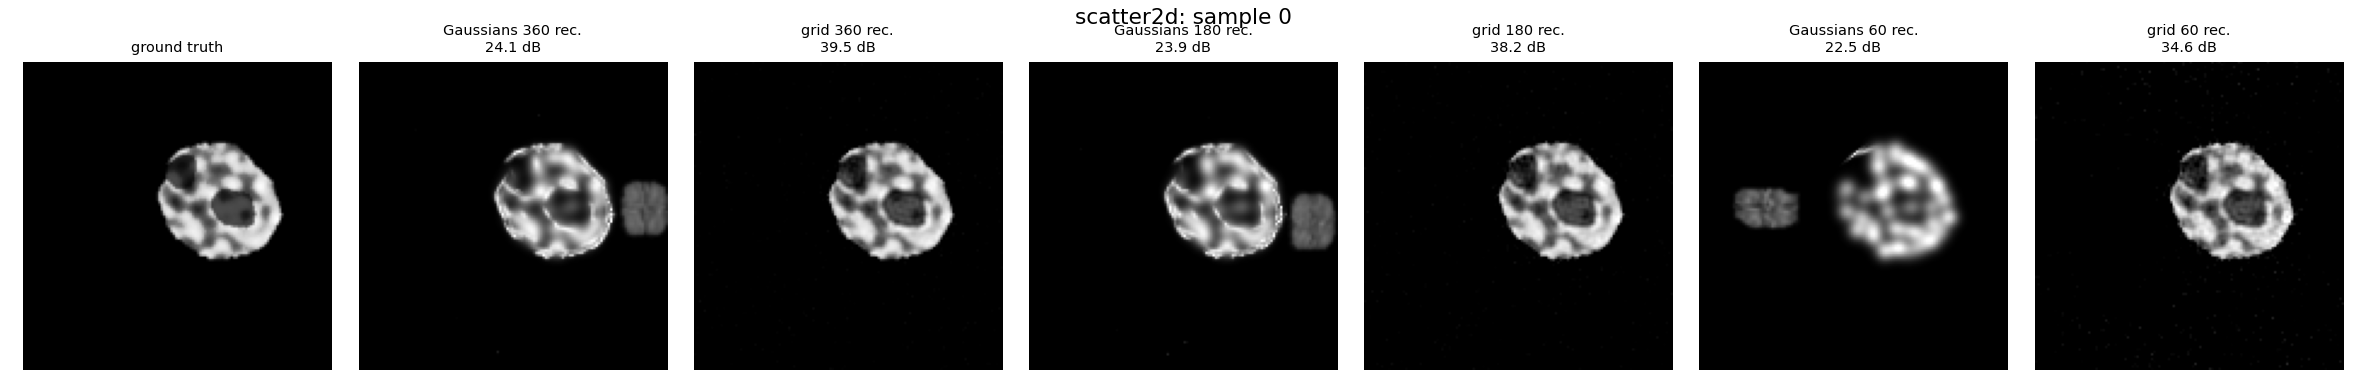
\includegraphics[width=\linewidth]{scatter2d_ghost.png}\\[2pt]
  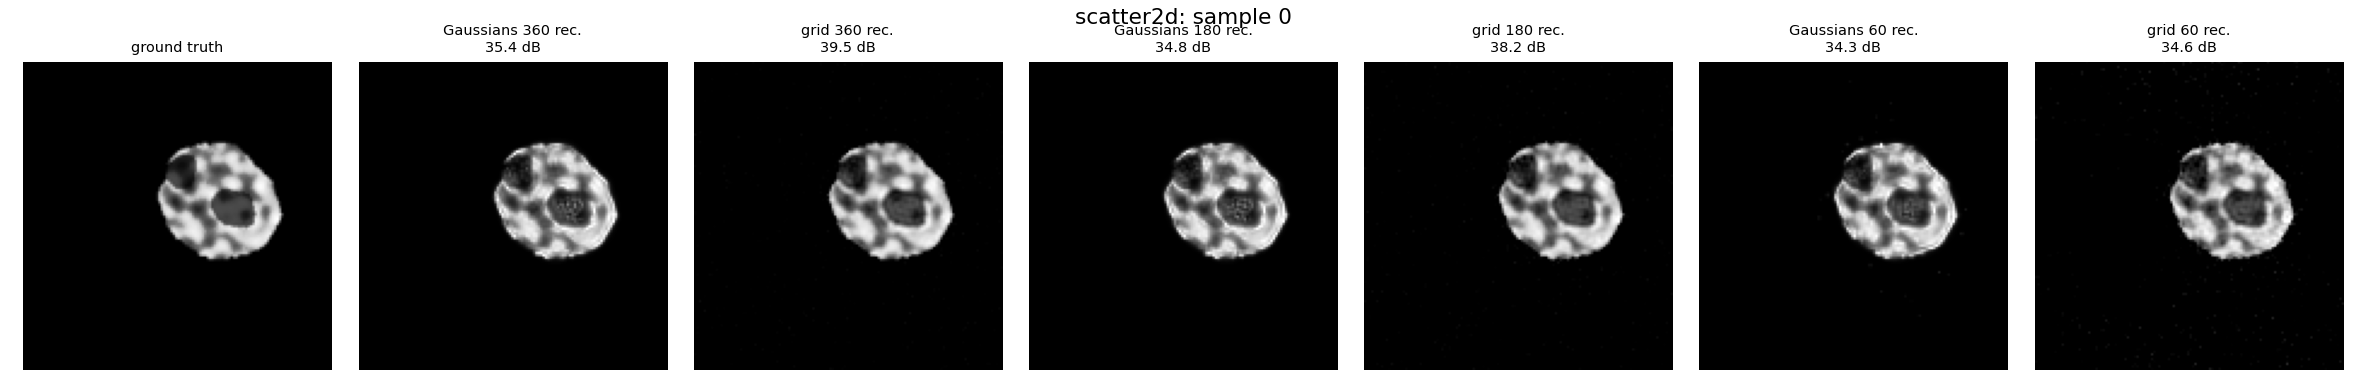
\includegraphics[width=\linewidth]{scatter2d_sparsity.png}
  \caption{Cell 0. Top: aggressive densification without regularisation produces a ghost copy beside the cell.
  Bottom: with the sparsity term ($\lambda=0.3$) the ghost is gone. Columns: ground truth, then Gaussian and pixel
  reconstructions at 360, 180 and 60 receivers.}
  \label{fig:ghost}
\end{figure}

\section{3D inverse scattering}
\label{sec:s3d}
On synthetic nuclei (Table~\ref{tab:s3d}, Figure~\ref{fig:s3d}) Gaussians are almost unaffected by the number of
receivers (40.6--40.9\,dB), while the voxel grid degrades from 44.1 to 37.3\,dB and becomes speckled. With 60
receivers Gaussians are better on all three volumes (+3.6\,dB on average) and have higher SSIM at every receiver
count.

The real CytoPacq nuclei from BBBC024 reverse this picture. The voxel grid reaches 35--42\,dB, while Gaussians stay at
27--28\,dB regardless of the number of receivers or the sparsity term. Figure~\ref{fig:s3d_bbbc} shows the reason: the
BBBC024 volumes are binary masks with sharp nucleus boundaries, and a sum of smooth Gaussians reproduces each
nucleus with a soft edge and a faint bright rim. The error is concentrated at the boundaries and is a
representation limit (the PSNR does not change with the receiver count), not a measurement limit. In SSIM, which is
less sensitive to edge error, Gaussians with sparsity (0.955) still beat the unregularised voxel grid (0.936) at 60
receivers, but not the voxel grid with the same sparsity (0.971). Together with the synthetic result this gives a
clear rule: Gaussians help when the object is smooth, and hurt when it is piecewise constant with sharp edges.

\begin{table}[h]
  \centering
  \caption{3D inverse scattering, $32\times128\times128$ volumes (PSNR dB / SSIM, mean of 3 volumes).}
  \label{tab:s3d}
  \resizebox{\linewidth}{!}{%
  \begin{tabular}{llccc}
    \toprule
    Volumes & Method & 360 receivers & 180 receivers & 60 receivers \\
    \midrule
    \multirow{2}{*}{Synthetic nuclei} & Gaussians & 40.8 / \textbf{0.994} & 40.6 / \textbf{0.994} & \textbf{40.9 / 0.988} \\
                                      & Voxel grid & \textbf{44.1} / 0.987 & \textbf{41.5} / 0.977 & 37.3 / 0.932 \\
    \midrule
    \multirow{4}{*}{BBBC024 (CytoPacq)} & Gaussians & 27.9 / 0.967 & 27.6 / 0.965 & 27.0 / 0.943 \\
                                         & Voxel grid & \textbf{41.8} / 0.989 & \textbf{40.3} / 0.980 & \textbf{35.3} / 0.936 \\
                                         & Gaussians + sparsity, $\lambda=0.3$ & 28.4 / 0.974 & 28.4 / 0.974 & 27.4 / 0.955 \\
                                         & Voxel grid + sparsity, $\lambda=0.3$ & 38.5 / \textbf{0.996} & 38.0 / \textbf{0.995} & 34.4 / \textbf{0.971} \\
    \bottomrule
  \end{tabular}}
\end{table}

\begin{figure}[h]
  \centering
  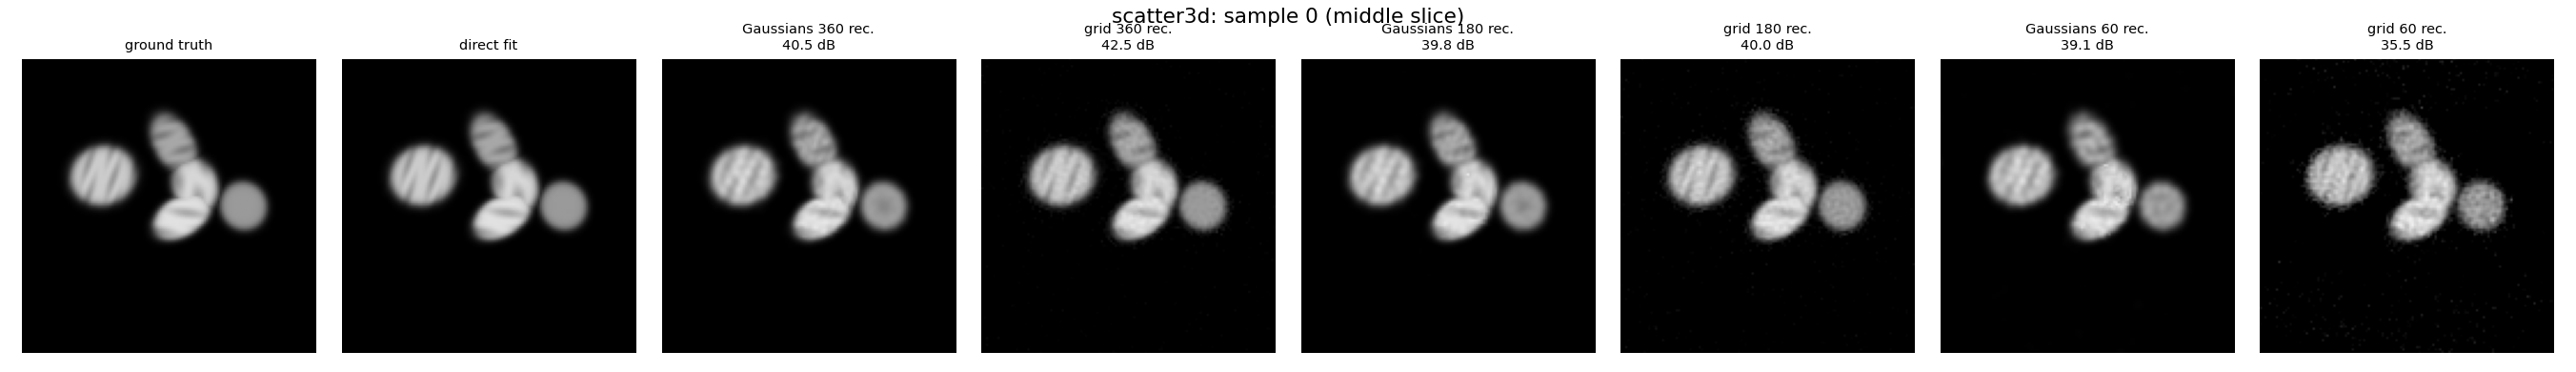
\includegraphics[width=\linewidth]{scatter3d_first.png}
  \caption{Middle slice of synthetic volume 0: ground truth, direct fit, then Gaussian and voxel reconstructions at
  360, 180 and 60 receivers.}
  \label{fig:s3d}
\end{figure}

\begin{figure}[h]
  \centering
  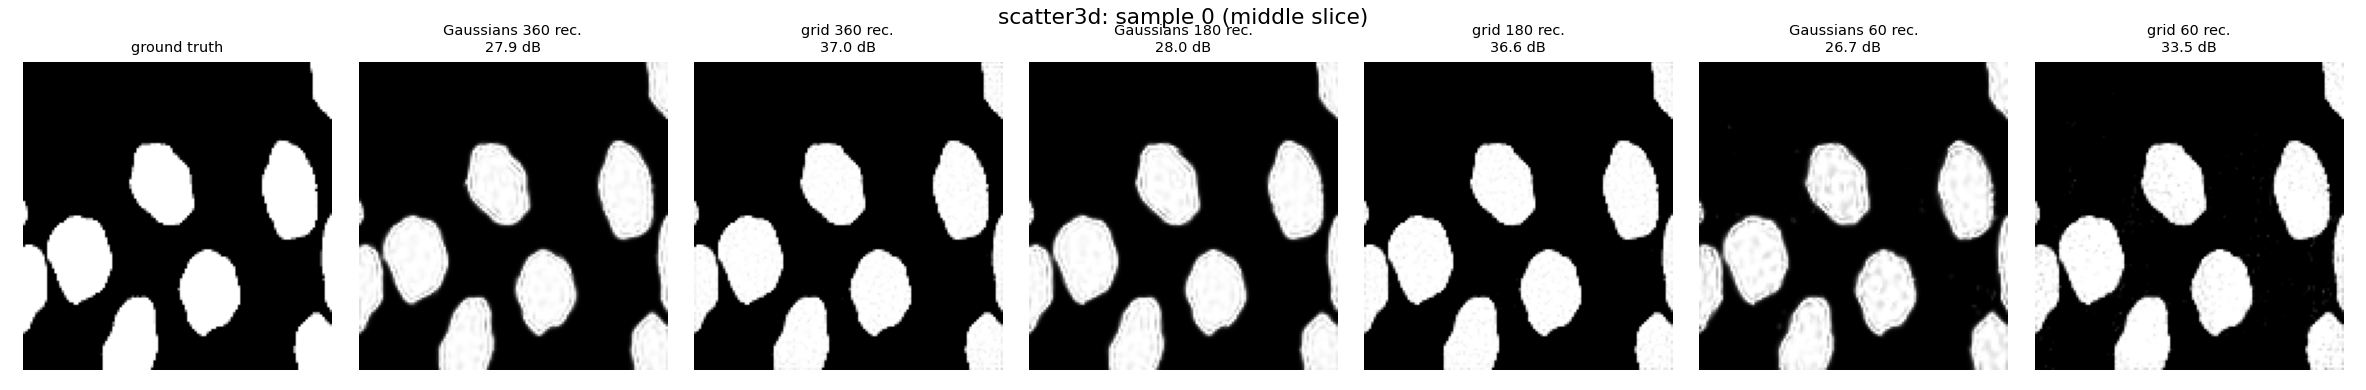
\includegraphics[width=\linewidth]{scatter3d_bbbc024.png}
  \caption{Middle slice of BBBC024 volume 0 (sparsity $\lambda=0.3$): ground truth, then Gaussian and voxel
  reconstructions at 360, 180 and 60 receivers. Gaussians soften the sharp nucleus boundaries and leave a faint rim.}
  \label{fig:s3d_bbbc}
\end{figure}

\section{4D Gaussians for Navier--Stokes}
Table~\ref{tab:ns} reports PSNR on held-out frames, with observed-frame PSNR in brackets. Static Gaussians reach only
about 17\,dB: the flow changes too much over 21 frames for one fixed field. A deformation network adds about 10\,dB.
Without regularisation, Mamba fits the observed frames much better than the MLP (36.1 vs.\ 30.3\,dB with full
observations), but on held-out frames the two are within 0.3\,dB: Mamba's extra capacity is spent memorising
observed times.

The final runs add the temporal smoothness term ($\lambda_T=1$). With 10\% of pixels observed, Mamba now generalises
clearly better than the MLP: 25.4 vs.\ 23.0\,dB on held-out frames, better on each of the three sequences
(+2.2, +2.0 and +2.9\,dB), and 2.3\,dB better than unregularised Mamba. The MLP is unchanged by the term, and the MLP
reconstructions show streak artefacts where data are sparse (Figure~\ref{fig:ns_smooth}). With full observations
all deformation models are within about 1\,dB (MLP 27.4, Mamba 27.2\,dB). The bidirectional Mamba fits observed frames
best but does not improve held-out frames (25.1 and 26.4\,dB) and doubles the training time. Mamba is about nine
times slower than the MLP (28 vs.\ 3\,min per sequence) because of its sequential pure-PyTorch scan.

\begin{table}[h]
  \centering
  \caption{4D Navier--Stokes, PSNR (dB) on held-out frames; observed-frame PSNR in brackets (mean of 3 sequences).
  ``+ smooth'' = temporal smoothness $\lambda_T=1$ (final runs).}
  \label{tab:ns}
  \resizebox{\linewidth}{!}{%
  \begin{tabular}{lcccc}
    \toprule
    Observed pixels & Static & MLP (4DGS-style) & Mamba & Bidirectional Mamba \\
    \midrule
    100\% & 17.0 (16.8) & 27.6 (30.3) & \textbf{27.9} (36.1) & -- \\
    100\% + smooth & -- & 27.4 (30.6) & 27.2 (35.2) & 26.4 (\textbf{36.5}) \\
    10\%  & 16.0 (15.9) & 23.2 (24.0) & 23.1 (27.7) & -- \\
    10\% + smooth & -- & 23.0 (24.1) & \textbf{25.4} (28.9) & 25.1 (\textbf{29.6}) \\
    \midrule
    Training time per sequence & 3\,min & 3\,min & 15--28\,min & 52\,min \\
    \bottomrule
  \end{tabular}}
\end{table}

\begin{figure}[h]
  \centering
  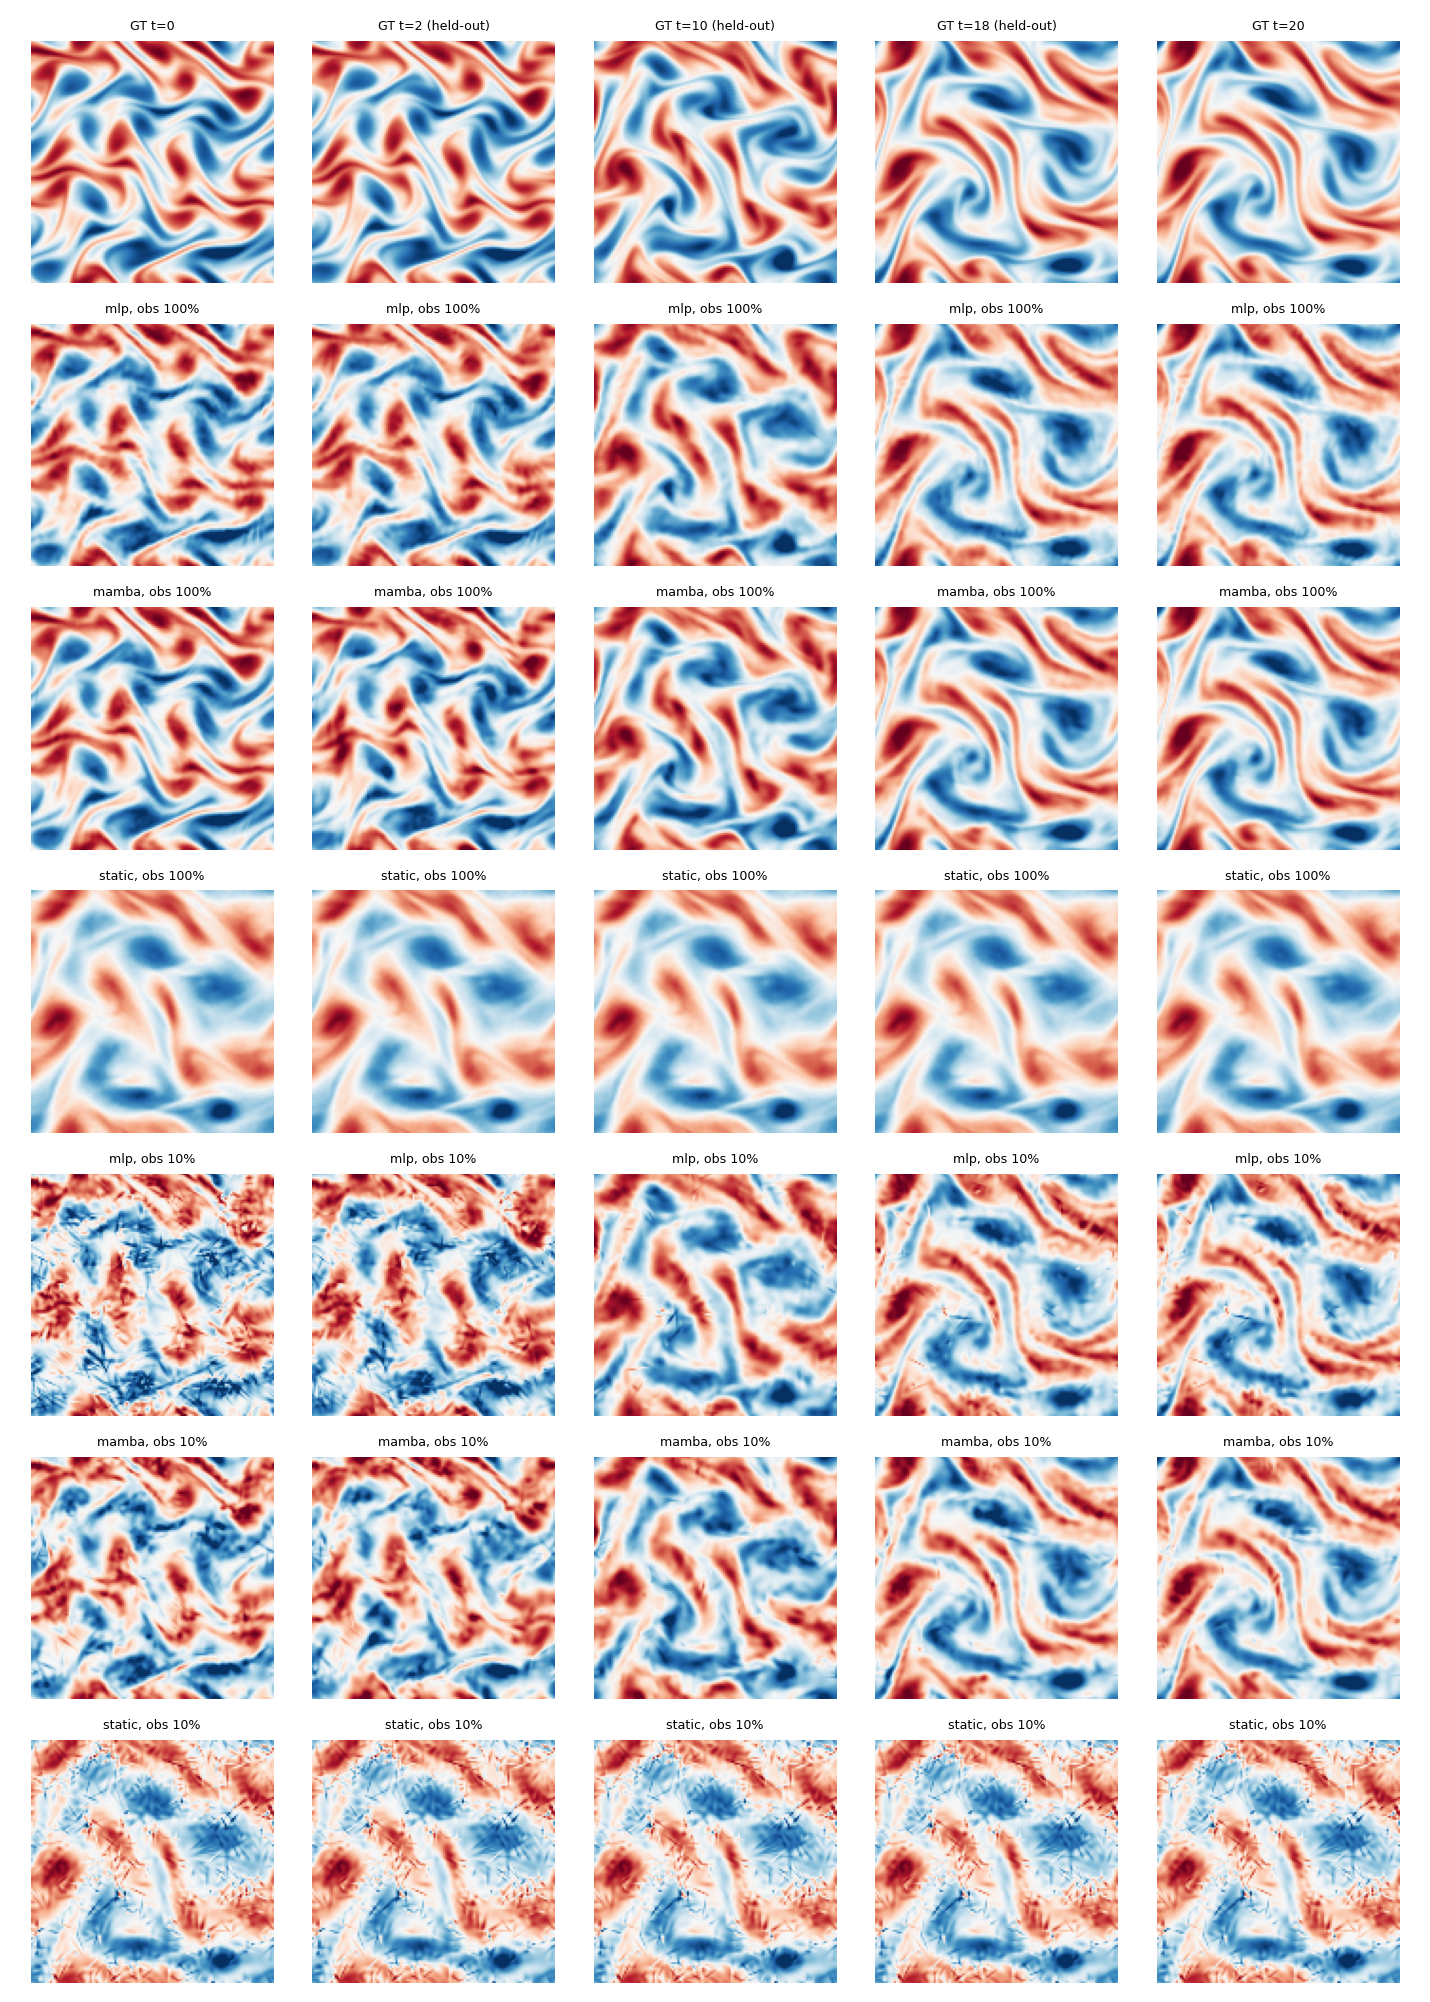
\includegraphics[width=0.85\linewidth]{ns4d_first.png}
  \caption{Initial runs: vorticity of sequence 0 at five times (held-out frames marked). Rows: ground truth, then
  MLP, Mamba and static models with 100\% and 10\% of pixels observed.}
  \label{fig:ns}
\end{figure}

\begin{figure}[h]
  \centering
  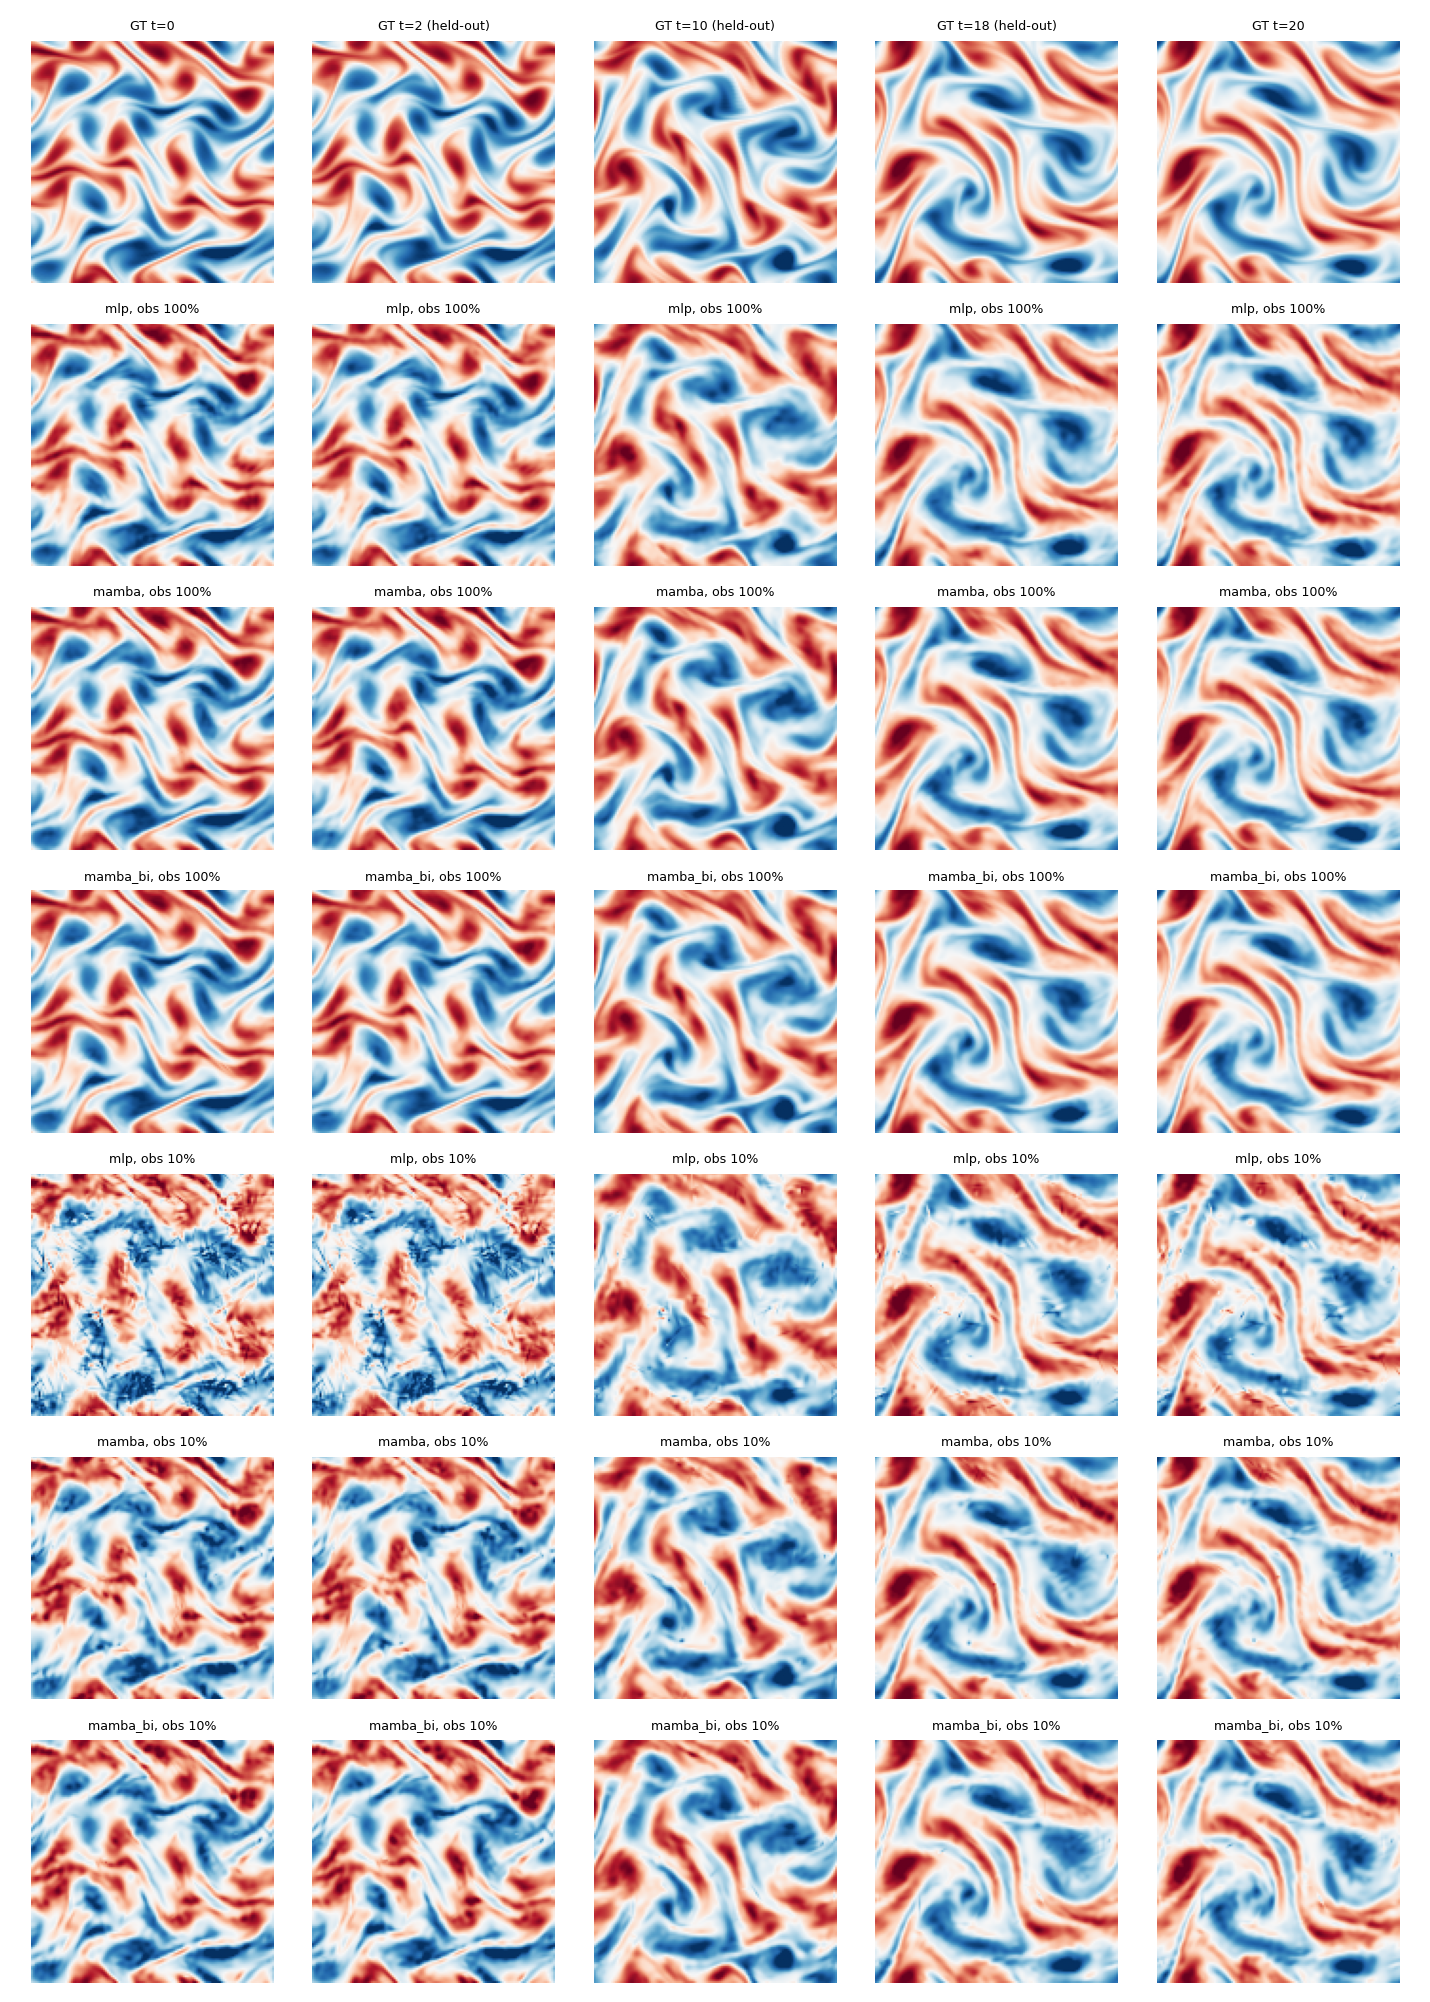
\includegraphics[width=0.75\linewidth]{ns4d_smooth.png}
  \caption{Final runs with temporal smoothness: ground truth, then MLP, Mamba and bidirectional Mamba with 100\% and
  10\% of pixels observed. With 10\% observations the MLP shows streaks; Mamba stays coherent.}
  \label{fig:ns_smooth}
\end{figure}

\section{Answers to the research questions}
\begin{description}
  \item[RQ1] Partly. On smooth 3D volumes Gaussians are more robust than voxels to scarce measurements (+3.6\,dB at 60
  receivers). On real, sharp-edged BBBC024 nuclei and on textured 2D cells the grid is better in PSNR; a grid with
  the same sparsity prior also matches or beats Gaussians in SSIM. The benefit depends on the object matching the
  smooth Gaussian prior.
  \item[RQ2] Adaptive densification can populate the operator's null space with ghost structures; a sparsity term on
  total intensity prevents them and is required for Gaussians.
  \item[RQ3] Yes: canonical Gaussians plus a deformation network reconstruct the flow at held-out times, about 10\,dB
  better than static Gaussians, from full or 10\% observations.
  \item[RQ4] Yes, when observations are sparse and the model is regularised in time: Mamba with temporal smoothness
  beats the MLP by 2.4\,dB on held-out frames with 10\% observations. With full observations there is no gain, and the
  bidirectional variant adds cost without benefit.
\end{description}
